
\begin{figure}
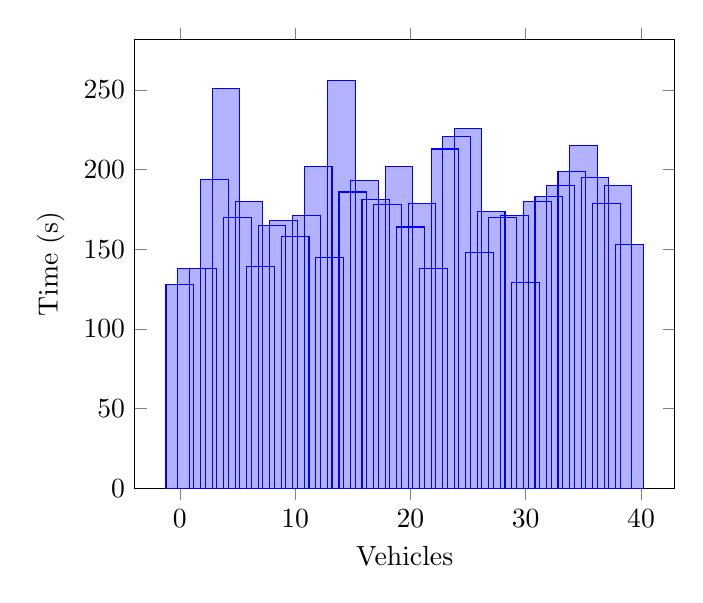
\begin{tikzpicture}
\begin{axis}[
legend style={anchor=west},
xlabel=Vehicles,
ylabel=Time (s),
ymin=0,
ybar,
]
\addplot coordinates {
(0, 128)
(1, 138)
(2, 138)
(3, 194)
(4, 251)
(5, 170)
(6, 180)
(7, 139)
(8, 165)
(9, 168)
(10, 158)
(11, 171)
(12, 202)
(13, 145)
(14, 256)
(15, 186)
(16, 193)
(17, 181)
(18, 178)
(19, 202)
(20, 164)
(21, 179)
(22, 138)
(23, 213)
(24, 221)
(25, 226)
(26, 148)
(27, 174)
(28, 170)
(29, 171)
(30, 129)
(31, 180)
(32, 183)
(33, 190)
(34, 199)
(35, 215)
(36, 195)
(37, 179)
(38, 190)
(39, 153)
};

\end{axis}
\end{tikzpicture}
\label{tik:0:2_O, 2_O.-60, 4_S, 5_S, 5_S.-30, 7_S, 7_S.-25, 11_S, 11_S.-50, 13_S, 15_N, 17_S, 17_S.-60, 18_S}
\caption{0 percent diving with GSC on route $2_O, 2_O.-60, 4_S, 5_S, 5_S.-30, 7_S, 7_S.-25, 11_S, 11_S.-50, 13_S, 15_N, 17_S, 17_S.-60, 18_S$}
\end{figure}
